\documentclass[tikz,border=12pt]{standalone}
\usepackage[T1]{fontenc}
\usepackage{tgheros}
\usepackage{sfmath}
\usepackage{amsmath}
% % \usepackage{fontawesome5} (Removed for publication-grade academic typography) (Removed for publication-grade academic typography)
\usepackage{tikz}
\usetikzlibrary{arrows.meta,positioning,shapes.geometric,fit,backgrounds,calc}
\usepackage{xcolor}

\renewcommand{\familydefault}{\sfdefault}

% Harvard Crimson & ETH Zurich Color Palette
\definecolor{harvardcrimson}{HTML}{A51C30}
\definecolor{ethdarkblue}{HTML}{1F407A}
\definecolor{ethblue}{HTML}{215CAF}
\definecolor{ethpetrol}{HTML}{007A87}
\definecolor{ethbronze}{HTML}{B87333}
\definecolor{ethslate}{HTML}{475569}
\definecolor{cardbg}{HTML}{F8FAFC}
\definecolor{cardborder}{HTML}{CBD5E1}

\begin{document}
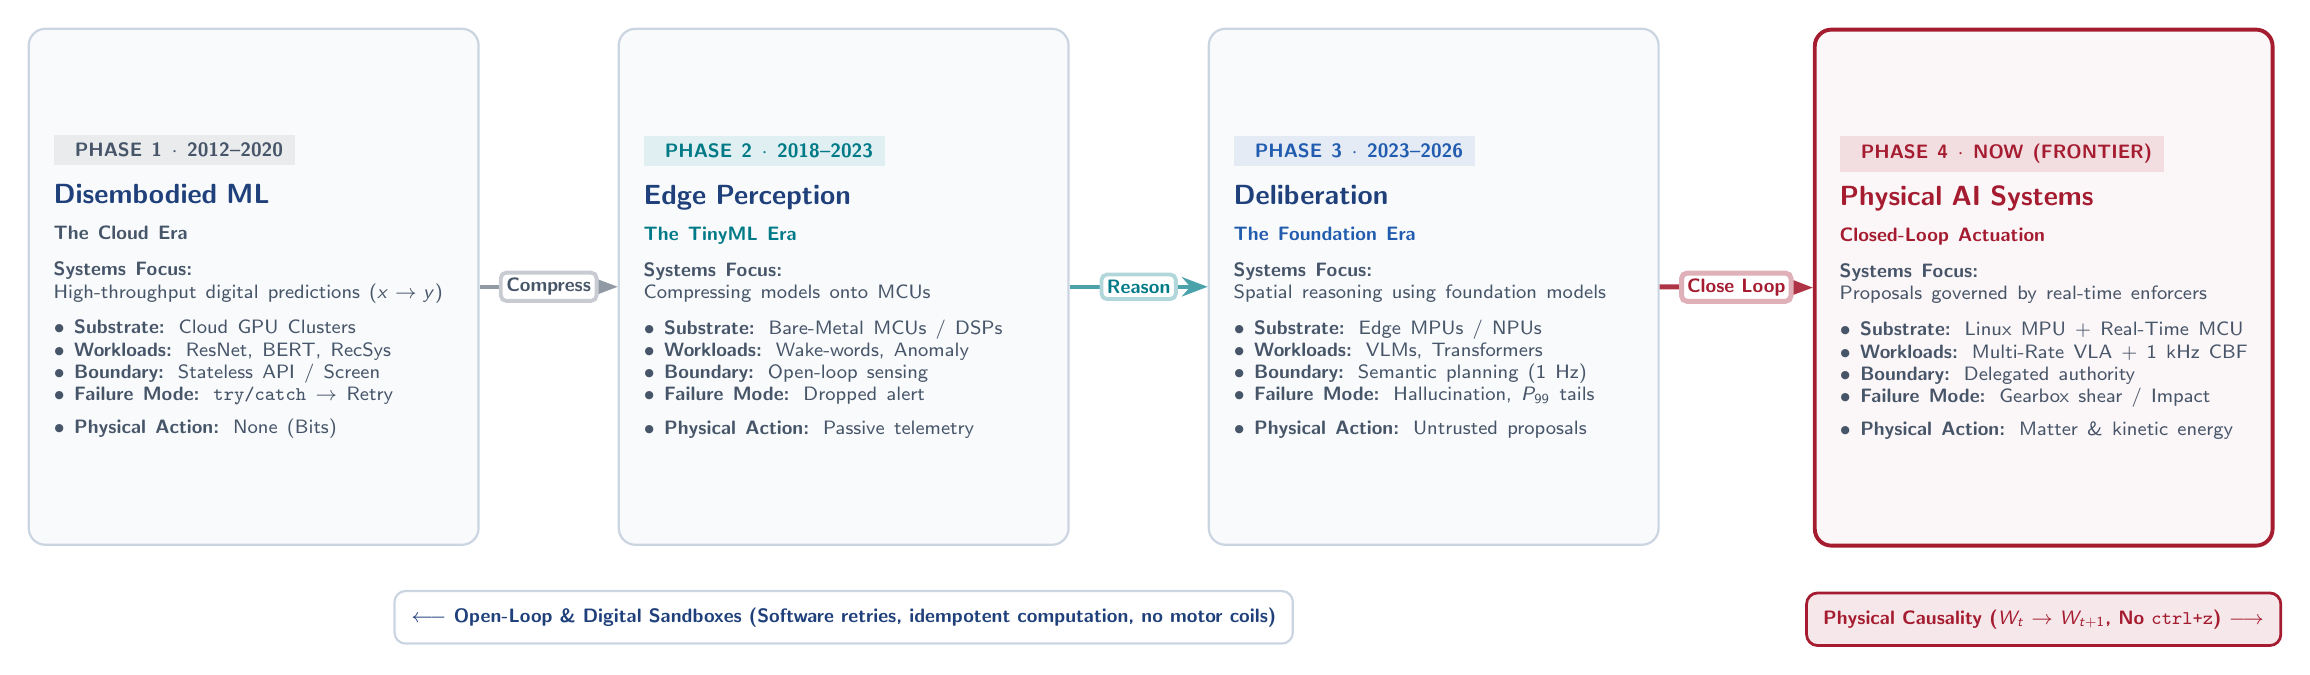
\begin{tikzpicture}[
  font=\sffamily,
  >=Stealth,
  card/.style={
    draw=cardborder,
    fill=cardbg,
    rounded corners=6pt,
    line width=0.8pt,
    text width=2.00in,
    minimum height=2.58in,
    inner sep=9pt,
    align=left,
    anchor=north
  },
  frontiercard/.style={
    draw=harvardcrimson,
    fill=harvardcrimson!4,
    rounded corners=6pt,
    line width=1.4pt,
    text width=2.04in,
    minimum height=2.58in,
    inner sep=9pt,
    align=left,
    anchor=north
  },
  arrowpill/.style={
    font=\sffamily\bfseries\scriptsize,
    fill=white,
    inner sep=2pt,
    rounded corners=2pt
  }
]

  % --- Phase 1: Disembodied ML ---
  \node[card] (p1) at (0,0) {
    {\scriptsize\bfseries\color{ethslate}\colorbox{ethslate!12}{\, PHASE 1 $\cdot$ 2012--2020\,}}\\[5pt]
    {\normalsize\bfseries\color{ethdarkblue}Disembodied ML}\\[1pt]
    {\scriptsize\bfseries\color{ethslate}The Cloud Era}\\[5pt]
    {\scriptsize\color{ethslate}\raggedright
    \textbf{Systems Focus:}\\
    High-throughput digital predictions ($x \to y$)\\[5pt]
    $\bullet$ \textbf{Substrate:} Cloud GPU Clusters\\
    $\bullet$ \textbf{Workloads:} ResNet, BERT, RecSys\\
    $\bullet$ \textbf{Boundary:} Stateless API / Screen\\
    $\bullet$ \textbf{Failure Mode:} \texttt{try/catch} $\to$ Retry\\
    $\bullet$ \textbf{Physical Action:} None (Bits)
    }
  };

  % --- Phase 2: Edge Perception ---
  \node[card] (p2) at (2.95in,0) {
    {\scriptsize\bfseries\color{ethpetrol}\colorbox{ethpetrol!12}{\, PHASE 2 $\cdot$ 2018--2023\,}}\\[5pt]
    {\normalsize\bfseries\color{ethdarkblue}Edge Perception}\\[1pt]
    {\scriptsize\bfseries\color{ethpetrol}The TinyML Era}\\[5pt]
    {\scriptsize\color{ethslate}\raggedright
    \textbf{Systems Focus:}\\
    Compressing models onto MCUs\\[5pt]
    $\bullet$ \textbf{Substrate:} Bare-Metal MCUs / DSPs\\
    $\bullet$ \textbf{Workloads:} Wake-words, Anomaly\\
    $\bullet$ \textbf{Boundary:} Open-loop sensing\\
    $\bullet$ \textbf{Failure Mode:} Dropped alert\\
    $\bullet$ \textbf{Physical Action:} Passive telemetry
    }
  };

  % --- Phase 3: Generative Deliberation ---
  \node[card] (p3) at (5.90in,0) {
    {\scriptsize\bfseries\color{ethblue}\colorbox{ethblue!12}{\, PHASE 3 $\cdot$ 2023--2026\,}}\\[5pt]
    {\normalsize\bfseries\color{ethdarkblue}Deliberation}\\[1pt]
    {\scriptsize\bfseries\color{ethblue}The Foundation Era}\\[5pt]
    {\scriptsize\color{ethslate}\raggedright
    \textbf{Systems Focus:}\\
    Spatial reasoning using foundation models\\[5pt]
    $\bullet$ \textbf{Substrate:} Edge MPUs / NPUs\\
    $\bullet$ \textbf{Workloads:} VLMs, Transformers\\
    $\bullet$ \textbf{Boundary:} Semantic planning ($1\text{ Hz}$)\\
    $\bullet$ \textbf{Failure Mode:} Hallucination, $P_{99}$ tails\\
    $\bullet$ \textbf{Physical Action:} Untrusted proposals
    }
  };

  % --- Phase 4: Physical AI Systems ---
  \node[frontiercard] (p4) at (8.95in,0) {
    {\scriptsize\bfseries\color{harvardcrimson}\colorbox{harvardcrimson!15}{\, PHASE 4 $\cdot$ NOW (FRONTIER)\,}}\\[5pt]
    {\normalsize\bfseries\color{harvardcrimson}Physical AI Systems}\\[1pt]
    {\scriptsize\bfseries\color{harvardcrimson}Closed-Loop Actuation}\\[5pt]
    {\scriptsize\color{ethslate}\raggedright
    \textbf{Systems Focus:}\\
    Proposals governed by real-time enforcers\\[5pt]
    $\bullet$ \textbf{Substrate:} Linux MPU + Real-Time MCU\\
    $\bullet$ \textbf{Workloads:} Multi-Rate VLA + 1 kHz CBF\\
    $\bullet$ \textbf{Boundary:} Delegated authority\\
    $\bullet$ \textbf{Failure Mode:} Gearbox shear / Impact\\
    $\bullet$ \textbf{Physical Action:} Matter \& kinetic energy
    }
  };

  % Transition Arrows with White Badge Pills
  \draw[->, line width=1.4pt, ethslate!60] (p1.east) -- node[pos=0.5, arrowpill, text=ethslate, draw=ethslate!30]{ Compress} (p2.west);
  \draw[->, line width=1.4pt, ethpetrol!70] (p2.east) -- node[pos=0.5, arrowpill, text=ethpetrol, draw=ethpetrol!30]{ Reason} (p3.west);
  \draw[->, line width=1.8pt, harvardcrimson!90] (p3.east) -- node[pos=0.5, arrowpill, text=harvardcrimson, draw=harvardcrimson!35]{ Close Loop} (p4.west);

  % Bottom Epistemic Divider Bar
  \node[draw=cardborder, fill=white, rounded corners=4pt, line width=0.8pt, inner sep=6pt, anchor=north, font=\sffamily\scriptsize\bfseries, text=ethdarkblue] 
    at ($(p1.south)!0.5!(p3.south) - (0, 0.22in)$) {
      $\longleftarrow$  \textbf{Open-Loop \& Digital Sandboxes} (Software retries, idempotent computation, no motor coils)
    };
  \node[draw=harvardcrimson, fill=harvardcrimson!10, rounded corners=4pt, line width=1pt, inner sep=6pt, anchor=north, font=\sffamily\scriptsize\bfseries, text=harvardcrimson] 
    at ($(p4.south) - (0, 0.22in)$) {
       \textbf{Physical Causality} ($W_t \to W_{t+1}$, No \texttt{ctrl+z}) $\longrightarrow$
    };

\end{tikzpicture}
\end{document}
